\documentclass[a4paper,11pt]{article}
\usepackage[czech]{babel}
\usepackage[T1]{fontenc}
\usepackage[utf8]{inputenc} 
\usepackage{hyperref}
\usepackage{graphicx}

\newcommand{\mail}{\href{mailto:jan.lochman@icloud.com}{jan.lochman@icloud.com}}

\newcommand{\cvut}{Czech Technical University in Prague}
\newcommand{\fjfi}{Faculty of Nuclear Sciences and Physical Engineering} 

\newcommand{\MyQuote}[2]{
  \begin{flushleft}
    \textit{\quotation{#1}}
  \end{flushleft}
  \begin{flushright}
    #2
  \end{flushright}
  \vspace{10mm}
}

\newenvironment{mytable2}[1][\unskip] 
{
\def\savedcaption{\caption{#1}}
\begin{table}[h]
\centering
\begin{tabular}{lr} 
}
{ 
\end{tabular} 
\savedcaption
\end{table} 
}



\title{Dokumentace LOM}
\date{\today}
\author{Pokusny Kralik, \mail}

\begin{document}


\maketitle
\tableofcontents 
\clearpage

\section{Uvod} 

Lorem ipsum dolor sit amet, consectetuer adipiscing elit. Etiam dui sem, fermentum vitae, sagittis id, malesuada in, quam. Nullam sapien sem, ornare ac, nonummy non, lobortis a enim. Integer imperdiet lectus quis justo. Proin mattis lacinia justo. Sed ut perspiciatis unde omnis iste natus error sit voluptatem accusantium doloremque laudantium, totam rem aperiam, eaque ipsa quae ab illo inventore veritatis et quasi architecto beatae vitae dicta sunt explicabo. Morbi leo mi, nonummy eget tristique non, rhoncus non leo. Etiam bibendum elit eget erat. Nullam at arcu a est sollicitudin euismod. Duis aute irure dolor in reprehenderit in voluptate velit esse cillum dolore eu fugiat nulla pariatur. Sed convallis magna eu sem. Maecenas sollicitudin. Aliquam ante. Pellentesque ipsum. Nunc tincidunt ante vitae massa. Nullam sit amet magna in magna gravida vehicula. Nulla non lectus sed nisl molestie malesuada. Aliquam ante. Pellentesque sapien. Integer imperdiet lectus quis justo.

Sed ac dolor sit amet purus malesuada congue. Nullam at arcu a est sollicitudin euismod. Nullam justo enim, consectetuer nec, ullamcorper ac, vestibulum in, elit. In enim a arcu imperdiet malesuada. Cum sociis natoque penatibus et magnis dis parturient montes, nascetur ridiculus mus. Suspendisse nisl. Sed convallis magna eu sem. Duis ante orci, molestie vitae vehicula venenatis, tincidunt ac pede. Phasellus et lorem id felis nonummy placerat. Nulla pulvinar eleifend sem. Ut enim ad minima veniam, quis nostrum exercitationem ullam corporis suscipit laboriosam, nisi ut aliquid ex ea commodi consequatur? Donec vitae arcu. Curabitur bibendum justo non orci. Aenean vel massa quis mauris vehicula lacinia.

Aliquam id dolor. Nulla non lectus sed nisl molestie malesuada. Nulla turpis magna, cursus sit amet, suscipit a, interdum id, felis. Nulla accumsan, elit sit amet varius semper, nulla mauris mollis quam, tempor suscipit diam nulla vel leo. Duis aute irure dolor in reprehenderit in voluptate velit esse cillum dolore eu fugiat nulla pariatur. Etiam dui sem, fermentum vitae, sagittis id, malesuada in, quam. Maecenas ipsum velit, consectetuer eu lobortis ut, dictum at dui. Duis aute irure dolor in reprehenderit in voluptate velit esse cillum dolore eu fugiat nulla pariatur. Proin pede metus, vulputate nec, fermentum fringilla, vehicula vitae, justo. Nam quis nulla.

Duis ante orci, molestie vitae vehicula venenatis, tincidunt ac pede. Etiam sapien elit, consequat eget, tristique non, venenatis quis, ante. Quisque tincidunt scelerisque libero. Nullam at arcu a est sollicitudin euismod. Maecenas sollicitudin. Integer malesuada. Fusce suscipit libero eget elit. Etiam neque. Fusce tellus odio, dapibus id fermentum quis, suscipit id erat. Sed ut perspiciatis unde omnis iste natus error sit voluptatem accusantium doloremque laudantium, totam rem aperiam, eaque ipsa quae ab illo inventore veritatis et quasi architecto beatae vitae dicta sunt explicabo. Fusce nibh. Duis viverra diam non justo. Duis risus. Integer pellentesque quam vel velit.

Aliquam erat volutpat. Ut enim ad minima veniam, quis nostrum exercitationem ullam corporis suscipit laboriosam, nisi ut aliquid ex ea commodi consequatur? Morbi scelerisque luctus velit. In enim a arcu imperdiet malesuada. Integer lacinia. Mauris dolor felis, sagittis at, luctus sed, aliquam non, tellus. Temporibus autem quibusdam et aut officiis debitis aut rerum necessitatibus saepe eveniet ut et voluptates repudiandae sint et molestiae non recusandae. Aliquam erat volutpat. Etiam ligula pede, sagittis quis, interdum ultricies, scelerisque eu. Fusce consectetuer risus a nunc.

\section{Vypoctove Hodnoty}

Vkladani tabulek je trosicku neprijemny, da se jednoduse stylovat. Asi
nejjednodussi je vytvorit pro to vlastni environment.

\begin{mytable2}[Titulek tabulky]
  prvni radek & hodnota \\
  druhy radek & hodnota \\ 
  mozno i podtrhnout & hodnota \\
  \hline
  1 & 2 \\
  \hline
\end{mytable2}


\begin{mytable2}[Dalsi tabulka]
  \hline
  prvni radek & hodnota \\
  \hline
  druhy radek & hodnota \\ 
  \hline
  mozno i podtrhnout & hodnota \\
  \hline
  1 & 2 \\
  \hline
\end{mytable2}

Mate oblibene styly vkladani textu? Neni problem, naprihlad citat se muze
vkladat takto

\MyQuote{What we observe is not nature itself, but nature exposed to our method of
questioning.}{Werner Heisenberg}

A styl vsech citatu se da jednoduse zmenit na jednom miste.


\section{Rozdeleni Zarizeni}

Dalsi uzasnou veci jsou pripravene prikazy. Ty jsou v souboru
\textit{slovnik.tex}. Napriklad mail, vcetne odkazu pro poslani, se vlozi
naprosto jednoduse, staci: \mail.

Vkladani fyzikalnich velicin? Jednoduche jako facka 1000\mh, 20\gc.

Predpripravene, casto pouzivane slovni spojeni? \soucProstTepla strechou.

Prikazy se daji pripravit s parametry, napriklad \tempWithTolerance{20}{1}. Nebo
vami casteji pouzivany \tempRangeMax{20}{26}

A prakticky jakakoliv casteji se opakovana fraze, jednotka, tabulka se da takhle
predpripravit. Predpripravit si ceskou frazi? Pak staci zmenit soubor s ceskymi
frazemi za soubor s anglickymi a je hotovo.

\section{Popis Jendotlivych VZT Zarizeni}

\section{Prilohy}

Sekce~\ref{sec:ukazkaObrazku} obsahuje obrazek~\ref{fig:testObrazek}.

\subsection{Ukazka vkladani obrazku}
\label{sec:ukazkaObrazku}

Latex sam rozhodne, kam obrazek vlozi.

\begin{figure}[t]
  \centering
  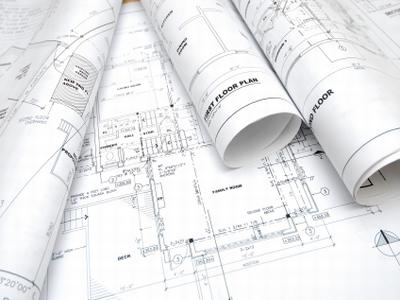
\includegraphics[width=0.5\textwidth]{obrazky/test.jpg}
  \caption{Nadpis k pokusnemu obrazku.}
  \label{fig:testObrazek}
\end{figure}



%================================================================================
% Tabulky
%================================================================================
\clearpage
\addcontentsline{toc}{section}{\listtablename}
\listoftables

%================================================================================
% Obrazky
%================================================================================
\clearpage
\addcontentsline{toc}{section}{\listfigurename}
\listoffigures
\end{document}
